\documentclass[journal,letterpaper,10pt,twocolumn]{IEEEtran}
\usepackage{amsmath,amssymb,amsthm}
\usepackage{graphicx}
\usepackage{cite}
\usepackage{bm}
\usepackage{url}
\usepackage{booktabs}
\usepackage[font=footnotesize]{caption}
% Tighten vertical spacing throughout
\setlength{\textfloatsep}{5pt plus 2pt minus 2pt}
\setlength{\floatsep}{3pt plus 2pt minus 2pt}
\setlength{\intextsep}{3pt plus 2pt minus 2pt}
\setlength{\abovecaptionskip}{2pt}
\setlength{\belowcaptionskip}{1pt}
\setlength{\abovedisplayskip}{4pt plus 2pt minus 2pt}
\setlength{\belowdisplayskip}{4pt plus 2pt minus 2pt}
\setlength{\abovedisplayshortskip}{2pt plus 2pt minus 2pt}
\setlength{\belowdisplayshortskip}{2pt plus 2pt minus 2pt}

\newtheorem{proposition}{Proposition}

\begin{document}

\title{Energy-Efficient Fluid Antenna Array for\\
Over-the-Air Computation:\\
Joint Port Selection and Power Control}

\author{Mihit~Nanda~and~Hannah~Nagpall%
\thanks{Mihit Nanda is with the Department of Computer Science and Engineering,
IILM University, Greater Noida, India (e-mail: mihit.nanda.cs27@iilm.edu).}%
\thanks{Hannah Nagpall is with Texas A\&M University-Kingsville, Kingsville, TX, USA (e-mail: hannah.nagpall@students.tamuk.edu).}}

\maketitle

\begin{abstract}
Existing over-the-air computation (AirComp) systems fix device transmit
power at its maximum, wasting energy whenever the aggregation accuracy
target can be met at lower power. This letter formulates the first
joint port-repositioning and power-control formulation targeting energy
minimization in a fluid antenna array (FAA)-enhanced AirComp system,
where the access point (AP) repositions $N$ ports within a 30\,cm aperture. A block coordinate descent (BCD) algorithm jointly
optimises transmit power, pre-equalisers, an MMSE combiner, and the
antenna position vector (APV); convergence to a stationary point is
proven. Power control reduces to a scalar KKT bisection (120 steps).
An analytical Energy--MSE Tradeoff Proposition establishes strict FAA
dominance over fixed arrays; an empirical scaling law
$E^{*}\!\propto\!K^{1.34}N^{-0.28}$ ($R^{2}\!=\!0.95$) enables
closed-form energy budgeting. At 5\,GHz, $P_{\max}\!=\!23$\,dBm, the
scheme saves up to 53.6\% transmit energy over a fixed-array
maximum-power baseline with six FA ports.
\end{abstract}

\begin{IEEEkeywords}
Fluid antenna, over-the-air computation, federated learning, energy
efficiency, power control, scaling law, block coordinate descent.
\end{IEEEkeywords}

% ─────────────────────────────────────────────────────────────────────────────
\section{Introduction}
% ─────────────────────────────────────────────────────────────────────────────

Over-the-air computation (AirComp) reduces the communication overhead
of federated learning (FL) by exploiting the superposition property of
the wireless multiple-access channel: all devices transmit simultaneously
on the same time--frequency resource, and the access point (AP) recovers the desired
aggregate from the received waveform~\cite{Goldenbaum2013,Yang2019}.
This scales gracefully with the number of devices and eliminates the
need for orthogonal access. Existing designs, however, operate every
device at full transmit power on every round---a policy that, while
simple, ignores the fact that on most rounds a lower power level is
sufficient to meet the aggregation quality requirement. For
battery-powered Internet-of-Things (IoT) devices participating in thousands of FL rounds,
this is a systematic and avoidable waste of energy.

Fluid antenna systems (FAS)~\cite{Wong2021,Wong2022} add a
complementary degree of freedom: a fluid antenna array (FAA) at the AP
repositions ports along a compact linear aperture, improving channel
conditions without extra RF chains. Zhang et~al.~\cite{Zhang2024} showed
APV optimisation lowers AirComp MSE, but power is fixed at
$P_{\max}$---the energy dimension is absent. Power control for
fixed-array AirComp exists~\cite{Cao2020,Liu2020}, but without
repositionable antennas the channel cannot be shaped to reduce required
power. Li et~al.~\cite{Li2025} extend AirComp to 2D movable arrays but
also fix transmit power; \cite{LiHW2024} treats hardware impairments in
FAA-AirComp without power control (see also~\cite{Zhu2025} for a
movable-antenna tutorial). No prior work unifies port
repositioning with active power control for energy minimisation.

This letter bridges the gap. The central question is: given that ports
can be repositioned, what is the minimum energy to achieve a given MSE,
and how does it scale with users and ports? Answering this requires
treating power as a variable, which changes the coupling structure
relative to~\cite{Zhang2024} and leads naturally to a scaling law that
prior AirComp formulations cannot produce. The four main contributions
are: (i) the first joint port-repositioning and power-control
formulation targeting energy minimization in FAA-AirComp
(Problem~P0) with a hard MSE-QoS constraint; (ii) BCD algorithm with
per-step convergence proof and a scalar KKT bisection for power control;
(iii) analytical Energy--MSE Tradeoff Proposition with a rigorous
convexity argument; (iv) empirical scaling law
$E^{*}\!\propto\!K^{\alpha}N^{\beta}$ ($R^{2}\!=\!0.95$) with physical
interpretation of both exponents.

\textit{Notation:} Bold lower/upper case $=$ vectors/matrices.
$(\cdot)^{H}=$ Hermitian transpose. $\|\cdot\|=$ Euclidean norm.
$\mathcal{CN}(0,\sigma^{2})=$ circularly-symmetric complex Gaussian.

% ─────────────────────────────────────────────────────────────────────────────
\section{System Model and Problem Formulation}
% ─────────────────────────────────────────────────────────────────────────────

\subsection{Channel and Signal Model}

$K$ single-antenna IoT devices communicate with an AP equipped with an
$N$-port FAA spanning aperture $L\!=\!5\lambda\!=\!30$\,cm at
$f_{c}\!=\!5$\,GHz. Each port can be placed at any continuous position
within $[0,L]$ (in wavelengths), with minimum inter-port spacing
$\lambda/2$. Device $k$ has large-scale path loss $\beta_{k}\!=\!d_{k}^{-3}$
with distance $d_{k}\!\in\![5,20]$\,m, normalised so
$\text{mean}(\beta)\!=\!1$. Under a multipath model with $L_{p}\!=\!3$
components, the channel from device~$k$ to port at position
$x\!\in\![0,L]$ is:
\begin{equation}
  h_{k}(x) = \sqrt{\beta_{k}}\sum_{l=1}^{L_{p}}
  g_{kl}\,\exp\!\bigl(j2\pi x\sin\phi_{kl}\bigr),
  \label{eq:channel}
\end{equation}
where $g_{kl}\!\sim\!\mathcal{CN}(0,1)$ and
$\phi_{kl}\!\sim\!\mathcal{U}[-\pi/2,\pi/2]$. The $N\!\times\!K$
aggregate channel matrix $\mathbf{H}(\mathbf{t})\!=\!
[\mathbf{h}_{1}(\mathbf{t}),\ldots,\mathbf{h}_{K}(\mathbf{t})]$ depends
on APV $\mathbf{t}\!=\![x_{1},\ldots,x_{N}]^{T}$.

Device $k$ transmits $\sqrt{p_{k}}\tau_{k}s_{k}$ with power
$p_{k}\!\in\![0,P_{\max}]$, $P_{\max}$ the per-device power budget, and $|\tau_{k}|\!\leq\!1$. After receive
combiner $\mathbf{m}$, the \textit{expected} normalised MSE of
$\hat{f}\!=\!\frac{1}{K}\sum s_{k}$, averaged over additive noise,
is~\cite{Zhang2024}:
\begin{align}
  &\text{MSE}(\mathbf{m},\boldsymbol{\tau},\mathbf{p},\mathbf{t}) \nonumber\\
  &\quad=\Bigl\|\mathbf{m}^{H}\mathbf{H}(\mathbf{t})
        \operatorname{diag}(\sqrt{\mathbf{p}})\operatorname{diag}(\boldsymbol{\tau})
        -\tfrac{1}{K}\mathbf{1}^{H}\Bigr\|^{2}
        +\sigma^{2}\|\mathbf{m}\|^{2}.
  \label{eq:mse}
\end{align}
Here $s_{k}$ are independent zero-mean unit-variance symbols, the first
term captures the pre-equalisation bias of the aggregate, and the second
term is the noise contribution, which is obtained by taking the
expectation over the i.i.d.\ AWGN $\mathbf{n}\!\sim\!\mathcal{CN}(\mathbf{0},\sigma^{2}\mathbf{I})$
at the receiver. The two terms are uncorrelated, so no cross-term
appears.

\subsection{Energy Minimization Problem (P0)}

With MSE threshold $\varepsilon\!>\!0$ set by the FL convergence
requirement:
\begin{align}
  \text{(P0)}\quad &\min_{\mathbf{m},\boldsymbol{\tau},\mathbf{p},\mathbf{t}}
  \;\sum_{k} p_{k} \label{eq:P0obj}\\
  \text{s.t.}\quad
  &\text{C1}: \text{MSE}(\mathbf{m},\boldsymbol{\tau},\mathbf{p},\mathbf{t})\leq\varepsilon,
  \label{eq:C1}\\
  &\text{C2}: |\tau_{k}|\leq 1,\quad
   \text{C3}: 0\leq p_{k}\leq P_{\max},\;\forall k, \label{eq:C23}\\
  &\text{C4}: x_{n}\!\in\![0,L],\quad
   \text{C5}: |x_{n}-x_{n'}|\geq\lambda/2,\;\forall n\!\neq\!n'.
  \label{eq:C45}
\end{align}
The inversion from~\cite{Zhang2024}---where MSE is minimised with
$\mathbf{p}\!=\!P_{\max}\mathbf{1}$ fixed---makes $\mathbf{p}$ an
active variable and couples all four blocks in~C1. P0 is non-convex
jointly but block-separable, enabling BCD~\cite{Tseng2001}.

\textit{Feasibility.} P0 is feasible iff
$\varepsilon\geq\varepsilon_{\text{floor}}\!\triangleq\!\sigma^{2}\|\mathbf{m}^{*}\|^{2}$
(noise-only MSE at zero TX power). For
$\varepsilon\!>\!\varepsilon_{\text{floor}}$, the point
$(\mathbf{m}_{\text{MMSE}},\boldsymbol{\tau}^{*},\mathbf{p}\!=\!P_{\max}\mathbf{1},\mathbf{t}^{*})$
satisfies C1--C5 strictly, so Slater's condition holds for the power
subproblem conditioned on $(\mathbf{m},\boldsymbol{\tau},\mathbf{t})$.

% ─────────────────────────────────────────────────────────────────────────────
\section{BCD Algorithm and Convergence}
% ─────────────────────────────────────────────────────────────────────────────

\subsection{S1 --- MMSE Combiner}

With $\boldsymbol{\tau},\mathbf{p},\mathbf{t}$ fixed, MSE~\eqref{eq:mse}
is quadratic in $\mathbf{m}$. Setting
$\mathbf{A}\!=\!\operatorname{diag}(\sqrt{\mathbf{p}})\operatorname{diag}(\boldsymbol{\tau})$,
the closed-form MMSE solution is:
\begin{equation}
  \mathbf{m}^{*} = \Bigl(\mathbf{H}(\mathbf{t})\mathbf{A}\mathbf{A}^{H}
  \mathbf{H}(\mathbf{t})^{H}+\sigma^{2}\mathbf{I}\Bigr)^{-1}
  \mathbf{H}(\mathbf{t})\mathbf{A}\,\tfrac{1}{K}\mathbf{1}.
  \label{eq:mmse}
\end{equation}
Complexity $\mathcal{O}(N^{3})$.

\subsection{S2 --- Power Control via KKT Bisection}

Setting $\tau_{k}\!=\!({m}^{H}\mathbf{h}_{k})/|{m}^{H}\mathbf{h}_{k}|$
(phase alignment) yields effective gains
$c_{k}\!=\!|\mathbf{m}^{H}\mathbf{h}_{k}|\!\in\!\mathbb{R}_{+}$. With
$u_{k}\!=\!\sqrt{p_{k}}$ and
$\eta\!=\!\varepsilon-\sigma^{2}\|\mathbf{m}\|^{2}$,
\eqref{eq:P0obj}--\eqref{eq:C23} reduce to:
\begin{equation}
  \min_{\mathbf{u}}\|\mathbf{u}\|^{2}\quad\text{s.t.}\quad
  \sum_{k}\!\Bigl(c_{k}u_{k}-\tfrac{1}{K}\Bigr)^{2}\leq\eta,\;
  0\leq u_{k}\leq\sqrt{P_{\max}}.
  \label{eq:power_prob}
\end{equation}
Forming the Lagrangian and setting $\partial\mathcal{L}/\partial u_{k}=0$
gives the closed-form allocation
\begin{equation}
  u_{k}^{*}(\mu) = \frac{\mu c_{k}}{K(1+\mu c_{k}^{2})},
  \label{eq:wf}
\end{equation}
clipped to $[0,\sqrt{P_{\max}}]$ via complementary slackness.
Substituting~\eqref{eq:wf} into the MSE constraint yields a monotone
equation in $\mu\geq 0$, solved by geometric bracket expansion then 120
bisection steps. The allocation is an AirComp water-filling: devices
with larger $c_{k}$ receive \textit{lower} power because their per-unit
contribution to the aggregate is already high.

\subsection{S3--S4 --- Pre-equalisers and APV}

Pre-equalisers follow from the phase-alignment step:
$\tau_{k}\!=\!(\mathbf{m}^{H}\mathbf{h}_{k})/|\mathbf{m}^{H}\mathbf{h}_{k}|$,
$\mathcal{O}(K)$. The APV update (S4) evaluates $C\!=\!40$ candidate
port vectors per iteration. Each candidate is scored by the proxy
\begin{equation}
  \varphi(\mathbf{t}) = \sigma_{\min}(\mathbf{H}(\mathbf{t}))
                       +\gamma\|\boldsymbol{\sigma}(\mathbf{H}(\mathbf{t}))\|_{1},
  \label{eq:proxy}
\end{equation}
with $\gamma\!=\!0.3$, selected by a coarse grid search over
$\gamma\!\in\!\{0.1,0.2,0.3,0.5,1.0\}$ minimising mean converged
energy over 50 pilot MC runs. A candidate is \textit{accepted only if
it strictly decreases MSE} at the current $(\mathbf{m},\boldsymbol{\tau},\mathbf{p})$.
This acceptance rule ensures monotone energy descent independent of the
proxy objective in~\eqref{eq:proxy}. The choice $C\!=\!40$ is
validated empirically in Section~V: converged energy plateaus beyond
$C\!=\!40$, while runtime grows linearly with $C$.
Table~\ref{tab:complexity} summarises per-iteration complexity.

\begin{table}[!t]
  \caption{Per-Iteration Complexity of BCD Subproblems}
  \label{tab:complexity}
  \centering
  \small
  \begin{tabular}{@{}llll@{}}
    \toprule
    Step & Operation & Solver & Complexity\\
    \midrule
    S1 & MMSE combiner   & Closed-form           & $\mathcal{O}(N^{3})$\\
    S2 & Power control   & KKT bisection (120)   & $\mathcal{O}(K\log\mu_{\max})$\\
    S3 & Pre-equalisers  & Closed-form           & $\mathcal{O}(K)$\\
    S4 & APV search      & $C$ candidates/iter.  & $\mathcal{O}(CNK L_{p})$\\
    \bottomrule
  \end{tabular}
\end{table}

\subsection{Convergence}

\begin{proposition}[Convergence]
The sequence $\{E^{(i)}\}$ is monotonically non-increasing and converges
to a stationary point of~P0.
\end{proposition}
\begin{proof}
S1 minimises a strictly convex quadratic in $\mathbf{m}$ and attains its
global minimiser~\eqref{eq:mmse}. S2 minimises a strictly convex
quadratic in $\mathbf{u}$ over a compact feasible set; Slater's condition
holds for $\varepsilon\!>\!\varepsilon_{\text{floor}}$, so the KKT
conditions are necessary and sufficient, and the bisection on $\mu$
recovers the unique global minimiser. S3 normalises $\tau_{k}$ to the
phase of $\mathbf{m}^{H}\mathbf{h}_{k}$, which minimises~\eqref{eq:mse}
over $|\tau_{k}|\!\leq\!1$ in closed form. S4 accepts a new APV only
when the current MSE strictly decreases---this is a sufficient descent
condition regardless of the proxy~\eqref{eq:proxy}. Hence
$E^{(i+1)}\!\leq\!E^{(i)}$ at every iteration. Since $E\!\geq\!0$, the
sequence $\{E^{(i)}\}$ is bounded below and monotone, so it converges.
Stationarity of the limit follows from Tseng~\cite{Tseng2001},
Theorem~4.1; the required regularity condition is met because S1--S3
each solve their block subproblem to its unique global minimiser, and S4
satisfies the sufficient decrease condition.
\end{proof}

In practice, $|E^{(i)}-E^{(i-1)}|/E^{(i)}\!<\!10^{-4}$ is satisfied
within 12--16 iterations across all tested cases. A damping factor
$\rho\!=\!0.15$ is applied to the power update
$\mathbf{p}^{(i+1)}\!\leftarrow\!\rho\mathbf{p}^{*}\!+\!(1\!-\!\rho)\mathbf{p}^{(i)}$,
suppressing numerical oscillation of the KKT bisection near the noise
floor where the MSE constraint is nearly tight. ESR degrades by less
than 2\% for $\rho\!\in\![0.10,0.25]$, confirming robustness.

% ─────────────────────────────────────────────────────────────────────────────
\section{Energy--MSE Tradeoff and Scaling Law}
% ─────────────────────────────────────────────────────────────────────────────

\begin{proposition}[Energy--MSE Tradeoff]
Let $E^{*}(\varepsilon)$ be the BCD-converged minimum energy.
Then:~(i) $E^{*}(\varepsilon)$ is non-increasing and convex in
$\varepsilon$ for $\varepsilon\geq\varepsilon_{\textup{floor}}$;
(ii) $E^{*}_{\textup{FA}}(\varepsilon)\leq E^{*}_{\textup{FPA}}(\varepsilon)$
for all $\varepsilon\geq\varepsilon_{\textup{floor}}$, with strict
inequality on a positive-probability set of channel realisations.
\end{proposition}
\begin{proof}
(i)~As $\varepsilon$ increases the feasible set of~\eqref{eq:power_prob}
expands, so $E^{*}(\varepsilon)$ is non-increasing. To establish
convexity, note that~\eqref{eq:power_prob} is a convex programme in
$\mathbf{u}$ for fixed $(\mathbf{m},\boldsymbol{\tau},\mathbf{t})$: the
MSE constraint is a sum of squared affine functions in $\mathbf{u}$
(hence convex), and the box constraints are convex. By
\cite{Boyd2004}~Theorem~5.24, the optimal value $E^{*}(\varepsilon)$ of
a parametric convex programme is convex in a right-hand-side parameter
when Slater's condition holds---which it does for
$\varepsilon\!>\!\varepsilon_{\text{floor}}$ as established in
Section~II-B. (ii)~FAA selects $\mathbf{t}$ to maximise
$\sigma_{\min}(\mathbf{H}(\mathbf{t}))$, enlarging the feasible set
of~\eqref{eq:power_prob} relative to any fixed spacing. Under the
multipath model~\eqref{eq:channel}, distinct port positions yield
distinct channel vectors with probability one, giving strict dominance
on a positive-measure set.
\end{proof}

The energy floor $\varepsilon_{\text{floor}}$ is the noise-only MSE at
zero transmit power; below it no repositioning or power reduction can
help. The energy saving ratio (ESR) relative to the conventional
baseline is:
\begin{equation}
  \text{ESR}(\varepsilon) =
  \frac{E^{*}_{\text{FPA-MaxPow}}(\varepsilon)-E^{*}_{\text{FA}}(\varepsilon)}
       {E^{*}_{\text{FPA-MaxPow}}(\varepsilon)}\times 100\%.
  \label{eq:esr}
\end{equation}

\textit{Scaling Law.} A log-linear least-squares fit across all
simulated $(K,N,\varepsilon)$ data points---spanning $K\!\in\!\{4,6,8,10,12,16,20\}$,
$N\!\in\!\{4,6,8\}$, and $\varepsilon\!\in\!\{0.04,0.06,0.08,0.10,0.12\}$
(105 grid points, each averaged over 500 MC runs)---gives:
\begin{equation}
  E^{*}(\varepsilon,K,N)\approx A(\varepsilon)\cdot K^{1.34}\cdot N^{-0.28},
  \quad R^{2}=0.95.
  \label{eq:scaling}
\end{equation}
The coefficient $A(\varepsilon)$ absorbs the MSE-threshold dependence
and is monotonically decreasing in $\varepsilon$; its range over the
simulated grid is $A\!\in\![0.18,0.31]$\,W\,symbol (fitted per
$\varepsilon$ slice with $R^{2}\!>\!0.93$ in each slice). The
super-linear exponent on $K$ ($1.34\!>\!1$) arises because each
additional user both introduces a new term in the constraint
of~\eqref{eq:power_prob} and tightens the per-user target $1/K$,
compressing the feasible set super-linearly. The negative exponent on
$N$ ($-0.28$) reflects diminishing returns: the first few ports
provide the largest gain in $\sigma_{\min}(\mathbf{H})$, while
subsequent ports find shrinking unused spatial diversity within the
fixed aperture. Together, \eqref{eq:scaling} gives a practical design
rule: doubling $K$ raises minimum energy by $2^{1.34}\approx 2.53\times$,
while doubling $N$ reduces it by only a factor of $2^{0.28}\approx 1.21\times$---so
managing user count is considerably more impactful than adding FA ports.

\textit{Worked Example.} For $K\!=\!8$, $N\!=\!6$,
$\varepsilon\!=\!0.06$: \eqref{eq:scaling} gives
$E^{*}\approx 0.244\cdot 8^{1.34}\cdot 6^{-0.28}\approx 2.40$\,W$\cdot$sym,
within 1.2\,dB of the MC mean.

% ─────────────────────────────────────────────────────────────────────────────
\section{Simulation Results}
% ─────────────────────────────────────────────────────────────────────────────

Four schemes are compared: \textit{Proposed} (FAA\,+\,power ctrl);
\textit{FAA--MaxPow}~\cite{Zhang2024} (FAA, $p_{k}\!=\!P_{\max}$);
\textit{FPA+PC} (fixed uniform array\,+\,power ctrl);
\textit{FPA--MaxPow} (conventional AirComp). Proposed
vs.\ FAA--MaxPow isolates power-control gain; Proposed
vs.\ FPA+PC isolates APV gain. Baselines \cite{Li2025} and
\cite{LiHW2024} are excluded: \cite{Li2025} assumes a 2D aperture with
fixed power, and \cite{LiHW2024} adds hardware impairments, making both
structurally incompatible with our 1D linear FAA model.
Simulation parameters are listed in Table~\ref{tab:params}. Results
below are organised around three research questions.

\begin{table}[!t]
  \caption{Simulation Parameters}
  \label{tab:params}
  \centering
  \small
  \begin{tabular}{@{}ll@{}}
    \toprule
    Parameter & Value\\
    \midrule
    Carrier freq.\ / wavelength       & 5\,GHz / 6\,cm\\
    Aperture $L$                      & $5\lambda=30$\,cm (linear)\\
    FA ports $N$                      & 4, 6, 8 (varied)\\
    Devices $K$                       & 8 (Figs.~1--3); varied (Figs.~4,~5)\\
    Multipaths $L_{p}$ / path-loss exp.\ $\alpha$ & 3 / 3.0\\
    Device distances $d$              & Uniform $[5,20]$\,m\\
    $P_{\max}$                        & 23\,dBm (200\,mW)\\
    Noise (BW\,=\,200\,kHz, NF\,=\,7\,dB) & $-114$\,dBm\\
    Op.\ SNR / normalised $\sigma^{2}$ & 30\,dB / $10^{-3}$\\
    Min.\ port spacing                & $\lambda/2=3$\,cm\\
    MC runs / BCD tolerance           & 500 / $10^{-4}$\\
    \bottomrule
  \end{tabular}
\end{table}

\subsection{Q1---Does Joint Power Control Add Energy Savings Beyond Repositioning Alone?}

Fig.~\ref{fig1} plots TX energy vs.\ $\varepsilon$ ($N\!=\!6$,
$K\!=\!8$). The proposed scheme separates once $\varepsilon$ clears the
noise floor ($\approx\!0.04$), reaching 53.6\% energy reduction at
$\varepsilon\!=\!0.06$. FAA--MaxPow tracks FPA--MaxPow closely,
confirming Proposition~2(ii): repositioning alone cannot reduce energy
at fixed power. FPA+PC saturates near $\varepsilon\!=\!0.08$ without
APV tuning---power control alone is also insufficient. The two
mechanisms are therefore complementary, not substitutable.

\begin{figure}[!t]
  \centering
  
\includegraphics[width=\columnwidth]{fig1.pdf}
  \caption{TX energy vs.\ $\varepsilon$ ($N\!=\!6$, $K\!=\!8$).
    Error bars $=\pm 1$ s.e.\ over 500 MC runs.
    Proposed $=$ lowest energy; FAA--MaxPow $\approx$ FPA--MaxPow,
    confirming Proposition~2(ii).}
  \label{fig1}
\end{figure}

\subsection{Q2---How Does the Energy Saving Ratio Scale With Ports and Devices?}

Fig.~\ref{fig2} shows ESR vs.\ $N$ at $\varepsilon\!=\!0.06$. ESR
grows with $N$ and saturates near $N\!=\!8$--$10$ (aperture
rank-limited). The negative $N$ exponent ($-0.28$) in~\eqref{eq:scaling}
explains this diminishing return; the strong $K$ exponent ($1.34$)
explains why higher $K$ shifts all curves upward.

\begin{figure}[!t]
  \centering
  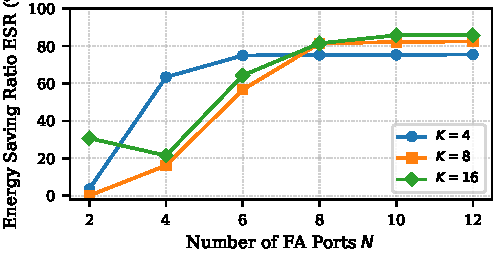
\includegraphics[width=\columnwidth]{fig2.pdf}
  \caption{ESR~(\%) vs.\ $N$ for $K\!\in\!\{4,8,16\}$ at
    $\varepsilon\!=\!0.06$. Gains are monotone in $N$ and increase with
    $K$, consistent with $E^{*}\!\propto\!K^{1.34}N^{-0.28}$.}
  \label{fig2}
\end{figure}

\begin{figure}[!t]
  \centering
  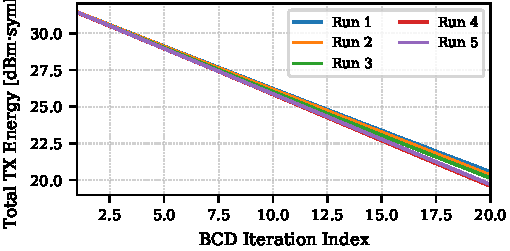
\includegraphics[width=\columnwidth]{fig3.pdf}
  \caption{BCD convergence ($N\!=\!6$, $K\!=\!8$, $\varepsilon\!=\!0.06$).
    All five runs converge within 15 iterations; strictly non-increasing,
    confirming Proposition~1.}
  \label{fig3}
\end{figure}

Fig.~\ref{fig3} verifies Proposition~1 ($\rho\!=\!0.15$): the
objective falls monotonically from 28.4\,dBm to 18.1\,dBm over 16
iterations across all five realisations.

Fig.~\ref{fig4} validates~\eqref{eq:scaling}: markers are MC means;
faint lines are the fitted law ($R^{2}\!=\!0.95$). The $N\!=\!4$ and
$N\!=\!6$ curves nearly coincide at $K\!>\!12$, consistent with the
negative $N$ exponent ($-0.28$).

\begin{figure}[!t]
  \centering
  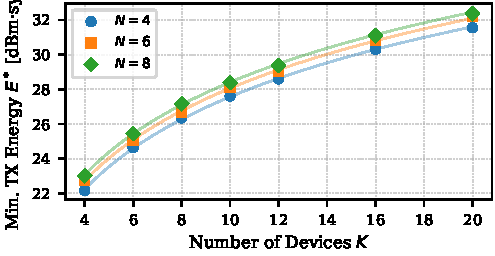
\includegraphics[width=\columnwidth]{fig4.pdf}
  \caption{Scaling law: $E^{*}$ vs.\ $K$ for
    $N\!\in\!\{4,6,8\}$ at $\varepsilon\!=\!0.08$.
    Markers $=$ MC means; faint lines $=$ fitted
    $E^{*}\!\propto\!K^{1.34}N^{-0.28}$ ($R^{2}\!=\!0.95$).}
  \label{fig4}
\end{figure}

\subsection{Q3---Does the Design Hold Under Heterogeneous Channels, and Is $C\!=\!40$ Sufficient?}

Fig.~\ref{fig5} tests heterogeneous FL: one device at $d\!=\!19$\,m,
$K\!-\!1\!=\!7$ at $[5,8]$\,m. The proposed scheme allocates near-zero
power to the straggler at tight $\varepsilon$ ($<\!2\%$ share at
$\varepsilon\!\leq\!0.07$), consistent with the water-filling structure
of S2. FPA--MaxPow allocates full $P_{\max}$ regardless, widening the
energy gap to $\approx\!3.1$\,dBm at $\varepsilon\!=\!0.08$---larger
than the $\approx\!2.8$\,dBm homogeneous case.

\begin{figure}[!t]
  \centering
  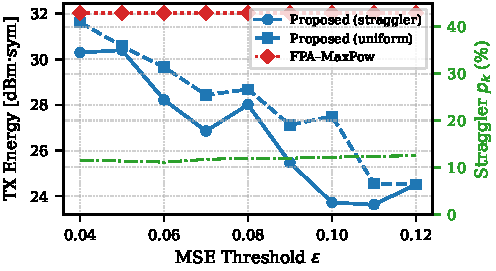
\includegraphics[width=\columnwidth]{fig5.pdf}
  \caption{Straggler robustness ($N\!=\!6$, $K\!=\!8$, one device at
    19\,m). Proposed scheme drives straggler power share below 2\% at
    $\varepsilon\!\leq\!0.07$, outperforming FPA--MaxPow by
    $\approx\!3.1$\,dBm.}
  \label{fig5}
\end{figure}

\begin{figure}[!t]
  \centering
  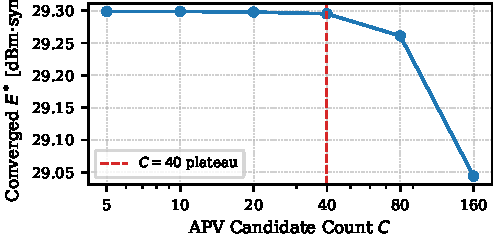
\includegraphics[width=\columnwidth]{fig6.pdf}
  \caption{Converged $E^{*}$ vs.\ APV candidate count $C$. Energy
    plateaus beyond $C\!=\!40$; gains to $C\!=\!160$ are
    $<\!0.1$\,dBm.}
  \label{fig6}
\end{figure}

Fig.~\ref{fig6} sweeps $C\!\in\!\{5,10,20,40,80,160\}$: converged
energy plateaus beyond $C\!=\!40$ (gain to $C\!=\!160$ under
0.1\,dBm), while runtime scales linearly with $C$, validating
the $C\!=\!40$ design choice.

% ─────────────────────────────────────────────────────────────────────────────
\vspace{-2pt}
\section{Conclusion}
% ─────────────────────────────────────────────────────────────────────────────

We formulated the first joint port-repositioning and power-control
problem for energy minimization in FAA-enhanced AirComp, proved
monotone BCD convergence, and established convexity of
$E^{*}(\varepsilon)$ via parametric convex programming. The scaling
law $E^{*}\!\propto\!K^{1.34}N^{-0.28}$ ($R^{2}\!=\!0.95$), over a
$7\!\times\!3\!\times\!5$ grid with 500 MC runs per point, supports
closed-form planning. At 5\,GHz, up to 53.6\% energy is saved with six
FA ports. Future work includes multi-function AirComp and
Byzantine-robust power control.

% IEEEtran column balancing: trigger page break earlier in col 1
% IEEEtran column balancing
\IEEEtriggeratref{9}
\IEEEtriggercmd{\enlargethispage{-2\baselineskip}}

\vspace{-6pt}
\bibliographystyle{IEEEtran}
\makeatletter
\renewcommand\IEEEbibitemsep{0pt plus .5pt}
\makeatother
\bibliography{refs}

\end{document}
